% this is a simplified version of
% https://github.com/yihui/knitr/blob/master/inst/examples/knitr-beamer.Rnw
\documentclass{beamer}\usepackage[]{graphicx}\usepackage[]{color}
%% maxwidth is the original width if it is less than linewidth
%% otherwise use linewidth (to make sure the graphics do not exceed the margin)
\makeatletter
\def\maxwidth{ %
  \ifdim\Gin@nat@width>\linewidth
    \linewidth
  \else
    \Gin@nat@width
  \fi
}
\makeatother

\definecolor{fgcolor}{rgb}{0.345, 0.345, 0.345}
\newcommand{\hlnum}[1]{\textcolor[rgb]{0.686,0.059,0.569}{#1}}%
\newcommand{\hlstr}[1]{\textcolor[rgb]{0.192,0.494,0.8}{#1}}%
\newcommand{\hlcom}[1]{\textcolor[rgb]{0.678,0.584,0.686}{\textit{#1}}}%
\newcommand{\hlopt}[1]{\textcolor[rgb]{0,0,0}{#1}}%
\newcommand{\hlstd}[1]{\textcolor[rgb]{0.345,0.345,0.345}{#1}}%
\newcommand{\hlkwa}[1]{\textcolor[rgb]{0.161,0.373,0.58}{\textbf{#1}}}%
\newcommand{\hlkwb}[1]{\textcolor[rgb]{0.69,0.353,0.396}{#1}}%
\newcommand{\hlkwc}[1]{\textcolor[rgb]{0.333,0.667,0.333}{#1}}%
\newcommand{\hlkwd}[1]{\textcolor[rgb]{0.737,0.353,0.396}{\textbf{#1}}}%
\let\hlipl\hlkwb

\usepackage{framed}
\makeatletter
\newenvironment{kframe}{%
 \def\at@end@of@kframe{}%
 \ifinner\ifhmode%
  \def\at@end@of@kframe{\end{minipage}}%
  \begin{minipage}{\columnwidth}%
 \fi\fi%
 \def\FrameCommand##1{\hskip\@totalleftmargin \hskip-\fboxsep
 \colorbox{shadecolor}{##1}\hskip-\fboxsep
     % There is no \\@totalrightmargin, so:
     \hskip-\linewidth \hskip-\@totalleftmargin \hskip\columnwidth}%
 \MakeFramed {\advance\hsize-\width
   \@totalleftmargin\z@ \linewidth\hsize
   \@setminipage}}%
 {\par\unskip\endMakeFramed%
 \at@end@of@kframe}
\makeatother

\definecolor{shadecolor}{rgb}{.97, .97, .97}
\definecolor{messagecolor}{rgb}{0, 0, 0}
\definecolor{warningcolor}{rgb}{1, 0, 1}
\definecolor{errorcolor}{rgb}{1, 0, 0}
\newenvironment{knitrout}{}{} % an empty environment to be redefined in TeX

\usepackage{alltt}
\usepackage{graphics}
\usepackage{url}
\usepackage{natbib}
\usepackage{bibentry}
\usepackage[english]{babel} %%remove tildes e.q. in bibliography

\bibliographystyle{apalike}
\usepackage{chngcntr}
\counterwithin*{footnote}{page}
\newcommand\footcite[1]{\footnote{\bibentry{#1}}\label{\thepage:#1}}
\newcommand\secondcite[1]{\textsuperscript{\ref{\thepage:#1}}}
% \def\newblock{\hskip .11em plus .33em minus .07em}
%\newcommand{\newblock}{}

\newcommand{\software}[1]{\textsl{#1}}
\newcommand\R{\software{R}}
% 
\newcommand\Bioconductor{\software{Bioconductor}}
\newcommand{\Rpackage}[1]{{\usebeamercolor[fg]{structure} \textsl{#1}}}
\newcommand\Biocpkg[1]{%
  {\href{http://bioconductor.org/packages/release/bioc/html/#1.html}%
    {\Rpackage{#1}}}}
\newcommand\Biocannopkg[1]{%
  {\href{http://bioconductor.org/packages/release/data/annotation/html/#1.html}%
    {\Rpackage{#1}}}}
\newcommand\Biocexptpkg[1]{%
  {\href{http://bioconductor.org/packages/release/data/experiment/html/#1.html}%
    {\Rpackage{#1}}}}
\newcommand\CRANpkg[1]{%
  {\href{http://cran.fhcrc.org/web/packages/#1/index.html}%
    {\Rpackage{#1}}}}
% 
\newcommand{\Rcode}[1]{\texttt{#1}}
\newcommand{\Rfunction}[1]{\Rcode{#1}}
\newcommand{\Robject}[1]{\Rcode{#1}}
\newcommand{\Rclass}[1]{\textit{#1}}
\IfFileExists{upquote.sty}{\usepackage{upquote}}{}
\begin{document}

\nobibliography{DSFBD}



\title{Data Structures for Biological Data in \R{}}
\author{Maarten van Iterson}
\date{\today}

\maketitle

% very important to use option [fragile] for frames containing code output!

% \begin{frame}
%   \frametitle{Table of Contents}
%   \tableofcontents
% \end{frame}

\section{Introduction}

\begin{frame}
  \frametitle{Goals}
  \begin{itemize}
  \item Which annotation packages are available within \Bioconductor{}\footcite{Gentleman2004}$^,$\footcite{Huber2015}
  \item How can we use these packages
  \item Get some idea of how these packages are implemented
  \item How to get annotation from online resources in \R{}
  \item Use \Bioconductor{} data/infra structure(s) for efficient handling of Biological data in \R{}
  \end{itemize}
\end{frame}

\begin{frame}
  \frametitle{Major types of annotation in \Bioconductor{}}
  Meta data/Annotation \Biocpkg{AnnotationDbi}\\
  \begin{itemize}
  \item Organism level: \Biocannopkg{org.Mm.eg.db}
  \item Platform level: \Biocannopkg{hgu133plus2.db}
  \item System-biology level: \Biocannopkg{GO.db} or \Biocannopkg{KEGG.db}
  \item Transcript centric annotations: \Biocpkg{GenomicFeatures}
  \end{itemize}
  \vfill
  Range data \Biocpkg{IRanges}, \Biocpkg{GenomicRanges} and \Biocpkg{GenomicFeatures}\\
  \begin{itemize}
  \item Genomic ranges: \Biocannopkg{TxDb.Hsapiens.UCSC.hg19.knownGene}
  \end{itemize}
  For example: annotation tracks from genome browsers or ChIP-seq data, a peak covering a certain region of the genome
\end{frame}

\begin{frame}
  \frametitle{Major types of annotation in \Bioconductor{}[CONT]}
  Sequence data: \Biocpkg{Biostrings} and \Biocpkg{BSgenome}
  \begin{itemize}
  \item Genomic sequences: \Biocannopkg{BSgenome.Hsapiens.UCSC.hg19}
  \end{itemize}
  For example: DNA/RNA sequences or motifs of transcription factor binding sites
  \vfill
  Query web-based resources for annotation and experimental data, e.g., ENCODE, ROADMAP, $\cdots$, tracks\\
  \begin{itemize}
  \item \Biocpkg{biomaRt} or \Biocpkg{AnnotationHub}
  \end{itemize}
  \vfill
  import of genomic data in various formats like BED, BAM, FASTQ, VCF, $\cdots$
  \begin{itemize}
  \item \Biocpkg{rtracklayer}, \Biocpkg{Rsamtools}, \Biocpkg{VariantAnnotation}
  \end{itemize}
\end{frame}

\section{Meta data/Annotation}

\begin{frame}
  \frametitle{Meta data/Annotation}
  \Bioconductor{} provides extensive annotation resource
  \begin{itemize}
  \item for associating microarray and other genomic data in real time with biological metadata from web databases such as GenBank, Entrez genes and PubMed
  \item covering a broad range of model organisms with support for different genomic builds
  \item updated every 6 months corresponding to the \Bioconductor{} release cycle
  \item customized annotation libraries can also be assembled
  \item implementations are based on \textbf{SQLite} with a number of higher-level interfaces e.g., using a simplified version of SQL queries
  \end{itemize}
\end{frame}

\begin{frame}[fragile]
  \frametitle{Example: Mapping between gene identifiers}
\begin{knitrout}\tiny
\definecolor{shadecolor}{rgb}{0.969, 0.969, 0.969}\color{fgcolor}\begin{kframe}
\begin{alltt}
\hlkwd{library}\hlstd{(org.Hs.eg.db)}
\hlstd{entrez_ids} \hlkwb{<-} \hlkwd{head}\hlstd{(}\hlkwd{keys}\hlstd{(org.Hs.eg.db,} \hlkwc{keytype}\hlstd{=}\hlstr{"ENTREZID"}\hlstd{))}
\hlstd{entrez_ids}
\end{alltt}
\begin{verbatim}
## [1] "1"  "2"  "3"  "9"  "10" "11"
\end{verbatim}
\begin{alltt}
\hlkwd{select}\hlstd{(org.Hs.eg.db,} \hlkwc{keys}\hlstd{=entrez_ids,} \hlkwc{columns}\hlstd{=}\hlkwd{c}\hlstd{(}\hlstr{"SYMBOL"}\hlstd{,}\hlstr{"ENSEMBL"}\hlstd{),} \hlkwc{keytype}\hlstd{=}\hlstr{"ENTREZID"}\hlstd{)}
\end{alltt}


{\ttfamily\noindent\itshape\color{messagecolor}{\#\# 'select()' returned 1:1 mapping between keys and columns}}\begin{verbatim}
##   ENTREZID SYMBOL         ENSEMBL
## 1        1   A1BG ENSG00000121410
## 2        2    A2M ENSG00000175899
## 3        3  A2MP1 ENSG00000256069
## 4        9   NAT1 ENSG00000171428
## 5       10   NAT2 ENSG00000156006
## 6       11   NATP            <NA>
\end{verbatim}
\end{kframe}
\end{knitrout}
\end{frame}

\begin{frame}
  \frametitle{Implementation}
  \begin{itemize}
  \item gene centric databases (ENTREZ GENE ID)
  \item out-of-memory data storage (SQLite )
  \item fast access to data subsets (lower-level interface using SQL)
  \item general and simple high-level interface \Rfunction{columns}, \Rfunction{keys}, \Rfunction{keytype} and \Rfunction{select}
  \end{itemize}
  \vfill
  Further reading: \Biocpkg{AnnotationDbi} vignettes:
  \begin{itemize}
  \item[]``AnnotationDbi: Introduction To Bioconductor Annotation Packages'' and
  \item[] ``How to use bimaps from the ".db" annotation packages''
  \end{itemize}
\end{frame}

\section{Range data}

\begin{frame}
  \frametitle{Range data\footcite{Lawrence2013}}
  Core packages \Biocpkg{IRanges}, \Biocpkg{GenomicRanges} and \Biocpkg{GenomicFeatures}
  \begin{itemize}
  \item directly supports more than 80 other \Bioconductor{} packages, including those for sequence analysis, differential expression analysis and visualization
  \item provide scalable data structures for representing annotated ranges on the genome, with special support for transcript structures, read alignments and coverage vectors.
  \item computational facilities include efficient algorithms for overlap and nearest neighbor detection, coverage calculation and
    other range operations.
  \end{itemize}
\end{frame}

\begin{frame}[fragile]
  \frametitle{Example: \Robject{Rle}, \Robject{IRanges} and
    \Robject{GRanges}}
\begin{knitrout}\tiny
\definecolor{shadecolor}{rgb}{0.969, 0.969, 0.969}\color{fgcolor}\begin{kframe}
\begin{alltt}
\hlstd{(seqnames} \hlkwb{<-} \hlkwd{Rle}\hlstd{(}\hlkwd{rep}\hlstd{(}\hlkwd{c}\hlstd{(}\hlstr{"chr1"}\hlstd{,} \hlstr{"chr2"}\hlstd{),} \hlkwd{c}\hlstd{(}\hlnum{1}\hlstd{,} \hlnum{3}\hlstd{))))}
\end{alltt}
\begin{verbatim}
## character-Rle of length 4 with 2 runs
##   Lengths:      1      3
##   Values : "chr1" "chr2"
\end{verbatim}
\begin{alltt}
\hlstd{(ranges} \hlkwb{<-} \hlkwd{IRanges}\hlstd{(}\hlnum{1}\hlopt{:}\hlnum{4}\hlstd{,} \hlkwc{end} \hlstd{=} \hlnum{11}\hlopt{:}\hlnum{14}\hlstd{,} \hlkwc{names} \hlstd{=} \hlkwd{head}\hlstd{(letters,} \hlnum{4}\hlstd{)))}
\end{alltt}
\begin{verbatim}
## IRanges object with 4 ranges and 0 metadata columns:
##         start       end     width
##     <integer> <integer> <integer>
##   a         1        11        11
##   b         2        12        11
##   c         3        13        11
##   d         4        14        11
\end{verbatim}
\begin{alltt}
\hlkwd{GRanges}\hlstd{(}\hlkwc{seqnames} \hlstd{= seqnames,} \hlkwc{ranges} \hlstd{= ranges,} \hlkwc{strand} \hlstd{=} \hlkwd{Rle}\hlstd{(}\hlkwd{strand}\hlstd{(}\hlkwd{c}\hlstd{(}\hlstr{"-"}\hlstd{,} \hlstr{"+"}\hlstd{)),}
    \hlkwd{c}\hlstd{(}\hlnum{1}\hlstd{,} \hlnum{3}\hlstd{)),} \hlkwc{GC} \hlstd{=} \hlkwd{seq}\hlstd{(}\hlnum{1}\hlstd{,} \hlnum{0}\hlstd{,} \hlkwc{length} \hlstd{=} \hlnum{4}\hlstd{))}
\end{alltt}
\begin{verbatim}
## GRanges object with 4 ranges and 1 metadata column:
##     seqnames    ranges strand |                GC
##        <Rle> <IRanges>  <Rle> |         <numeric>
##   a     chr1   [1, 11]      - |                 1
##   b     chr2   [2, 12]      + | 0.666666666666667
##   c     chr2   [3, 13]      + | 0.333333333333333
##   d     chr2   [4, 14]      + |                 0
##   -------
##   seqinfo: 2 sequences from an unspecified genome; no seqlengths
\end{verbatim}
\end{kframe}
\end{knitrout}
\end{frame}

\begin{frame}[fragile]
  \frametitle{Example: Obtain transcript structure}
\begin{knitrout}\tiny
\definecolor{shadecolor}{rgb}{0.969, 0.969, 0.969}\color{fgcolor}\begin{kframe}
\begin{alltt}
\hlkwd{library}\hlstd{(TxDb.Hsapiens.UCSC.hg19.knownGene)}
\hlkwd{library}\hlstd{(org.Hs.eg.db)}
\hlstd{kras_gene} \hlkwb{<-} \hlstd{org.Hs.egSYMBOL2EG}\hlopt{$}\hlstd{KRAS}
\hlstd{kras_gene}
\end{alltt}
\begin{verbatim}
## [1] "3845"
\end{verbatim}
\begin{alltt}
\hlstd{kras_exons} \hlkwb{<-} \hlkwd{exons}\hlstd{(TxDb.Hsapiens.UCSC.hg19.knownGene,}
\hlkwc{filter} \hlstd{=} \hlkwd{list}\hlstd{(}\hlkwc{gene_id} \hlstd{= kras_gene),}
\hlkwc{columns} \hlstd{=} \hlkwd{c}\hlstd{(}\hlstr{"tx_id"}\hlstd{,} \hlstr{"exon_id"}\hlstd{))}
\hlstd{kras_exons}
\end{alltt}
\begin{verbatim}
## GRanges object with 8 ranges and 2 metadata columns:
##       seqnames               ranges strand |             tx_id   exon_id
##          <Rle>            <IRanges>  <Rle> |     <IntegerList> <integer>
##   [1]    chr12 [25358180, 25362845]      - |       47893,47894    168446
##   [2]    chr12 [25368371, 25368494]      - |             47893    168447
##   [3]    chr12 [25378548, 25378707]      - |       47893,47894    168448
##   [4]    chr12 [25380168, 25380346]      - |       47893,47894    168449
##   [5]    chr12 [25386768, 25388160]      - |             47895    168450
##   [6]    chr12 [25398208, 25398329]      - | 47893,47894,47895    168451
##   [7]    chr12 [25403685, 25403854]      - |       47893,47894    168452
##   [8]    chr12 [25403698, 25403863]      - |             47895    168453
##   -------
##   seqinfo: 93 sequences (1 circular) from hg19 genome
\end{verbatim}
\end{kframe}
\end{knitrout}
\end{frame}

\begin{frame}
  \frametitle{Example: Obtain transcript structure}
  \begin{figure}
    \centering
    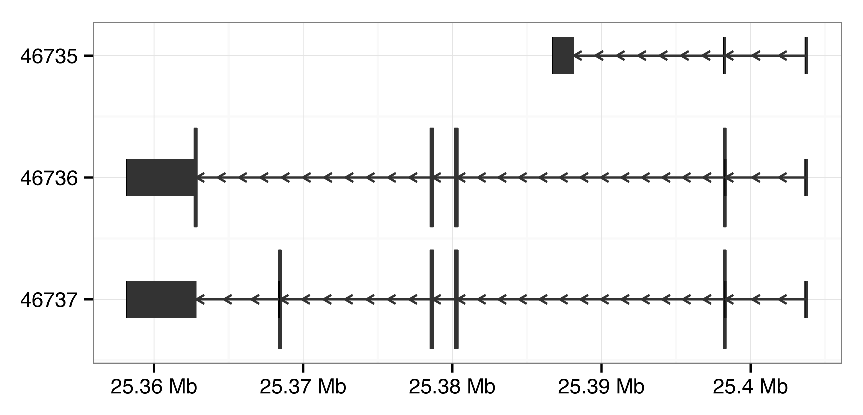
\includegraphics[width=\textwidth]{kras}
    \caption{Representation of the exons for the human KRAS gene, derived from the UCSC known gene annotation.}
  \end{figure}
\end{frame}

\begin{frame}
  \frametitle{Implementation}
  \Biocpkg{IRanges/GenomicRanges}
  \begin{itemize}
  \item Run-length-encoding for efficient storage of range data
  \item IRange object are derived from IntegerList a list of integer vectors
  \end{itemize}
  One of the most power features are finding overlapping regions between \Robject{IRanges} or \Robject{GRanges}
  \begin{itemize}
  \item \Rfunction{findOverlaps} function uses an efficient interval tree algorithm
  \item the algorithm supports several types of overlap, including those defined by Allen's Interval Algebra
  \item the one-time cost of constructing the interval tree is $O(n\log n)$, and queries are performed in logarithmic time
  \end{itemize}
\end{frame}

\section{Sequence data}

\begin{frame}[fragile]
  \frametitle{Sequence data}
  \Biocpkg{Biostrings} DNA, RNA and protein string manipulations
  \begin{itemize}
  \item counting and tabulating i.e., nucleotide frequencies
  \item sequence transformation and editing, i.e., translate DNA in RNA
  \item string matching/alignments, i.e., pattern matching
  \item I/O  functions, i.e. read/write FASTA files
  \end{itemize}
  \Biocpkg{BSgenome}
  \begin{itemize}
  \item 22 genomes with different builds e.g., H. sapiens has available builds:\\
\begin{knitrout}\tiny
\definecolor{shadecolor}{rgb}{0.969, 0.969, 0.969}\color{fgcolor}\begin{kframe}
\begin{verbatim}
##  [1] "BSgenome.Hsapiens.1000genomes.hs37d5"
##  [2] "BSgenome.Hsapiens.NCBI.GRCh38"       
##  [3] "BSgenome.Hsapiens.UCSC.hg17"         
##  [4] "BSgenome.Hsapiens.UCSC.hg17.masked"  
##  [5] "BSgenome.Hsapiens.UCSC.hg18"         
##  [6] "BSgenome.Hsapiens.UCSC.hg18.masked"  
##  [7] "BSgenome.Hsapiens.UCSC.hg19"         
##  [8] "BSgenome.Hsapiens.UCSC.hg19.masked"  
##  [9] "BSgenome.Hsapiens.UCSC.hg38"         
## [10] "BSgenome.Hsapiens.UCSC.hg38.masked"
\end{verbatim}
\end{kframe}
\end{knitrout}
  \item optionally \Biocpkg{BSgenome} package can be generated
  \end{itemize}
\end{frame}

\begin{frame}[fragile]
  \frametitle{Example: Obtain nucleotide frequency of Human chr 1/count number of MseI restriction sites}
\begin{knitrout}\tiny
\definecolor{shadecolor}{rgb}{0.969, 0.969, 0.969}\color{fgcolor}\begin{kframe}
\begin{alltt}
\hlkwd{library}\hlstd{(BSgenome.Hsapiens.UCSC.hg19)}
\hlstd{Hsapiens}\hlopt{$}\hlstd{chr1}
\end{alltt}
\begin{verbatim}
##   249250621-letter "DNAString" instance
## seq: NNNNNNNNNNNNNNNNNNNNNNNNNNNNNNNNNN...NNNNNNNNNNNNNNNNNNNNNNNNNNNNNNNNN
\end{verbatim}
\begin{alltt}
\hlkwd{alphabetFrequency}\hlstd{(Hsapiens}\hlopt{$}\hlstd{chr1)}
\end{alltt}
\begin{verbatim}
##        A        C        G        T        M        R        W        S 
## 65570891 47024412 47016562 65668756        0        0        0        0 
##        Y        K        V        H        D        B        N        - 
##        0        0        0        0        0        0 23970000        0 
##        +        . 
##        0        0
\end{verbatim}
\begin{alltt}
\hlstd{MseI} \hlkwb{<-} \hlstr{"TTAA"}
\hlkwd{countPattern}\hlstd{(MseI, Hsapiens}\hlopt{$}\hlstd{chr1)}
\end{alltt}
\begin{verbatim}
## [1] 1428207
\end{verbatim}
\end{kframe}
\end{knitrout}
\end{frame}

\begin{frame}
  \frametitle{Implementation}
  \begin{enumerate}
  \item use R external pointers to store the string data (references to C structures)
  \item use bit patterns to encode the string data
  \end{enumerate}
\end{frame}

\section{Online resources}
\begin{frame}
  \frametitle{Online resources}
  \begin{itemize}
  \item genome browsers like UCSC and Ensembl are a rich resource for annotation of biological data
  \item large Consortia make their data available through genome browser e.g., HapMap, ENCODE, ROADMAP, $\cdots$
  \end{itemize}
  \vfill
  \Biocpkg{biomaRt}, \Biocpkg{rtracklayer} and \Biocpkg{AnnotationHub}
  \begin{itemize}
  \item these packages provide easy access to public data repositories
  \item \Biocpkg{rtracklayer} has functionality to import various genomic data formats: GFF, BED, Bed15, bedGraph, WIG, BigWig
  \end{itemize}
\end{frame}

\begin{frame}[fragile]
  \frametitle{\Biocpkg{biomaRt} example: Get annotation from ENSEMBL}
\begin{knitrout}\tiny
\definecolor{shadecolor}{rgb}{0.969, 0.969, 0.969}\color{fgcolor}\begin{kframe}
\begin{alltt}
\hlkwd{library}\hlstd{(biomaRt)}
\hlstd{ensembl} \hlkwb{<-} \hlkwd{useMart}\hlstd{(}\hlstr{"ensembl"}\hlstd{,}\hlkwc{dataset}\hlstd{=}\hlstr{"hsapiens_gene_ensembl"}\hlstd{)}
\hlkwd{getBM}\hlstd{(}\hlkwc{attributes} \hlstd{=} \hlkwd{c}\hlstd{(}\hlstr{"hgnc_symbol"}\hlstd{,} \hlstr{"ensembl_gene_id"}\hlstd{) ,}
\hlkwc{filters} \hlstd{=} \hlstr{"entrezgene"}\hlstd{,}
\hlkwc{values} \hlstd{= entrez_ids,} \hlkwc{mart}\hlstd{= ensembl)}
\end{alltt}
\begin{verbatim}
##   hgnc_symbol ensembl_gene_id
## 1        A1BG ENSG00000121410
## 2        NAT2 ENSG00000156006
## 3         A2M ENSG00000175899
## 4       A2MP1 ENSG00000256069
## 5        NAT1 ENSG00000171428
\end{verbatim}
\end{kframe}
\end{knitrout}
\end{frame}

\begin{frame}[fragile]
  \frametitle{\Biocpkg{rtracklayer} example: Genome Segmentations track from ENCODE}
\begin{knitrout}\tiny
\definecolor{shadecolor}{rgb}{0.969, 0.969, 0.969}\color{fgcolor}\begin{kframe}
\begin{alltt}
\hlkwd{library}\hlstd{(rtracklayer)}
\hlstd{genomicSegmentation} \hlkwb{<-} \hlkwd{import}\hlstd{(}\hlstr{"wgEncodeAwgSegmentationChromhmmGm12878.bed"}\hlstd{,} \hlkwc{format}\hlstd{=}\hlstr{"BED"}\hlstd{)}
\hlkwd{head}\hlstd{(genomicSegmentation)}
\end{alltt}
\begin{verbatim}
## GRanges object with 6 ranges and 4 metadata columns:
##       seqnames         ranges strand |        name     score     itemRgb
##          <Rle>      <IRanges>  <Rle> | <character> <numeric> <character>
##   [1]     chr1 [    1, 10000]      * |       Quies      1000     #E1E1E1
##   [2]     chr1 [10001, 10400]      * |      FaireW      1000     #FFFC04
##   [3]     chr1 [10401, 15800]      * |         Low      1000     #C2D69A
##   [4]     chr1 [15801, 16000]      * |        Pol2      1000     #00B050
##   [5]     chr1 [16001, 16400]      * |       Gen3'      1000     #00B050
##   [6]     chr1 [16401, 16600]      * |        Elon      1000     #00B050
##                thick
##            <IRanges>
##   [1] [    1, 10000]
##   [2] [10001, 10400]
##   [3] [10401, 15800]
##   [4] [15801, 16000]
##   [5] [16001, 16400]
##   [6] [16401, 16600]
##   -------
##   seqinfo: 23 sequences from an unspecified genome; no seqlengths
\end{verbatim}
\end{kframe}
\end{knitrout}
\end{frame}

\begin{frame}[fragile]
  \frametitle{\Biocpkg{AnnotationHub} example: Obtain ROADMAP chromatin segmentation tracks}
\begin{knitrout}\tiny
\definecolor{shadecolor}{rgb}{0.969, 0.969, 0.969}\color{fgcolor}\begin{kframe}
\begin{alltt}
\hlkwd{library}\hlstd{(AnnotationHub)}
\hlstd{ah} \hlkwb{<-} \hlkwd{AnnotationHub}\hlstd{()}
\end{alltt}


{\ttfamily\noindent\itshape\color{messagecolor}{\#\# snapshotDate(): 2016-03-09}}\begin{alltt}
\hlkwd{query}\hlstd{(ah,} \hlkwd{c}\hlstd{(}\hlstr{"EpigenomeRoadMap"}\hlstd{,} \hlstr{"coreMarks"}\hlstd{))}
\end{alltt}
\begin{verbatim}
## AnnotationHub with 127 records
## # snapshotDate(): 2016-03-09 
## # $dataprovider: BroadInstitute
## # $species: Homo sapiens
## # $rdataclass: GRanges
## # additional mcols(): taxonomyid, genome, description, tags,
## #   sourceurl, sourcetype 
## # retrieve records with, e.g., 'object[["AH46856"]]' 
## 
##             title                             
##   AH46856 | E001_15_coreMarks_mnemonics.bed.gz
##   AH46857 | E002_15_coreMarks_mnemonics.bed.gz
##   AH46858 | E003_15_coreMarks_mnemonics.bed.gz
##   AH46859 | E004_15_coreMarks_mnemonics.bed.gz
##   AH46860 | E005_15_coreMarks_mnemonics.bed.gz
##   ...       ...                               
##   AH46978 | E125_15_coreMarks_mnemonics.bed.gz
##   AH46979 | E126_15_coreMarks_mnemonics.bed.gz
##   AH46980 | E127_15_coreMarks_mnemonics.bed.gz
##   AH46981 | E128_15_coreMarks_mnemonics.bed.gz
##   AH46982 | E129_15_coreMarks_mnemonics.bed.gz
\end{verbatim}
\end{kframe}
\end{knitrout}
\end{frame}

\begin{frame}[fragile]
  \frametitle{\Biocpkg{AnnotationHub} example: Obtain ROADMAP chromatin segmentation tracks[CONT]}
\begin{knitrout}\tiny
\definecolor{shadecolor}{rgb}{0.969, 0.969, 0.969}\color{fgcolor}\begin{kframe}
\begin{alltt}
\hlstd{ah[}\hlstr{'AH46982'}\hlstd{]}
\end{alltt}
\begin{verbatim}
## AnnotationHub with 1 record
## # snapshotDate(): 2016-03-09 
## # names(): AH46982
## # $dataprovider: BroadInstitute
## # $species: Homo sapiens
## # $rdataclass: GRanges
## # $title: E129_15_coreMarks_mnemonics.bed.gz
## # $description: 15 state chromatin segmentations from EpigenomeRoadMap ...
## # $taxonomyid: 9606
## # $genome: hg19
## # $sourcetype: BED
## # $sourceurl: http://egg2.wustl.edu/roadmap/data/byFileType/chromhmmSeg...
## # $sourcelastmodifieddate: 2013-10-11
## # $sourcesize: 2914216
## # $tags: EpigenomeRoadMap, chromhmmSegmentations, ChmmModels,
## #   coreMarks, E129, ENCODE2012, BONE.OSTEO, Osteoblast Primary
## #   Cells 
## # retrieve record with 'object[["AH46982"]]'
\end{verbatim}
\end{kframe}
\end{knitrout}
\end{frame}

\begin{frame}[fragile]
  \frametitle{\Biocpkg{AnnotationHub} example: Obtain ROADMAP chromatin segmentation tracks[CONT]}
\begin{knitrout}\tiny
\definecolor{shadecolor}{rgb}{0.969, 0.969, 0.969}\color{fgcolor}\begin{kframe}
\begin{alltt}
\hlstd{gr} \hlkwb{<-} \hlstd{ah[[}\hlstr{'AH46982'}\hlstd{]]}
\end{alltt}


{\ttfamily\noindent\itshape\color{messagecolor}{\#\# loading from cache '/home/mvaniterson/.AnnotationHub/52422'}}\begin{alltt}
\hlstd{gr}
\end{alltt}
\begin{verbatim}
## GRanges object with 511350 ranges and 4 metadata columns:
##            seqnames               ranges strand |        abbr
##               <Rle>            <IRanges>  <Rle> | <character>
##        [1]    chr10     [     1, 119600]      * |    15_Quies
##        [2]    chr10     [119601, 120200]      * |      1_TssA
##        [3]    chr10     [120201, 120400]      * |  2_TssAFlnk
##        [4]    chr10     [120401, 122000]      * |      5_TxWk
##        [5]    chr10     [122001, 122800]      * |      1_TssA
##        ...      ...                  ...    ... .         ...
##   [511346]     chrY [58984401, 58985800]      * |  8_ZNF/Rpts
##   [511347]     chrY [58985801, 58999400]      * |       9_Het
##   [511348]     chrY [58999401, 59001000]      * |    15_Quies
##   [511349]     chrY [59001001, 59033200]      * |       9_Het
##   [511350]     chrY [59033201, 59373400]      * |    15_Quies
##                           name        color_name  color_code
##                    <character>       <character> <character>
##        [1]       Quiescent/Low             White     #FFFFFF
##        [2]          Active TSS               Red     #FF0000
##        [3] Flanking Active TSS        Orange Red     #FF4500
##        [4]  Weak transcription         DarkGreen     #006400
##        [5]          Active TSS               Red     #FF0000
##        ...                 ...               ...         ...
##   [511346] ZNF genes & repeats Medium Aquamarine     #66CDAA
##   [511347]     Heterochromatin     PaleTurquoise     #8A91D0
##   [511348]       Quiescent/Low             White     #FFFFFF
##   [511349]     Heterochromatin     PaleTurquoise     #8A91D0
##   [511350]       Quiescent/Low             White     #FFFFFF
##   -------
##   seqinfo: 93 sequences (1 circular) from hg19 genome
\end{verbatim}
\end{kframe}
\end{knitrout}
\end{frame}

\begin{frame}
  \frametitle{Further Reading}
  \begin{itemize}
  \item  all vignettes: \textit{$>$ vignette("packageName")}
    \vfill
  \item \url{http://www.bioconductor.org/help/workflows/annotation/annotation/}
  \item \url{http://www.bioconductor.org/help/workflows/variants/}
  \item \url{http://www.bioconductor.org/help/workflows/annotation/AnnotatingRanges/}
    \vfill
  \item \url{http://www.ebi.ac.uk/training/sites/ebi.ac.uk.training/files/materials/2013/131021_HTS/genesandgenomes.pdf}
  \end{itemize}
\end{frame}

\end{document}
